% Created 2023-10-23 Mon 11:30
% Intended LaTeX compiler: pdflatex
\documentclass[t, 10pt, seahorse, bigger]{beamer}
\usepackage[utf8]{inputenc}
\usepackage[T1]{fontenc}
\usepackage{graphicx}
\usepackage{longtable}
\usepackage{wrapfig}
\usepackage{rotating}
\usepackage[normalem]{ulem}
\usepackage{amsmath}
\usepackage{amssymb}
\usepackage{capt-of}
\usepackage{hyperref}
\usetheme[height=20pt]{Rochester}
\usecolortheme{seahorse}
\author{Konstantinos Vasilakos}
\date{2023-10-23}
\title{Intelligent Beheamoths: live coding with Ltt}
\subtitle{CEAM  Conference, Moscow Conservatory Oct. 2023}
\hypersetup{
 pdfauthor={Konstantinos Vasilakos},
 pdftitle={Intelligent Beheamoths: live coding with Ltt},
 pdfkeywords={},
 pdfsubject={},
 pdfcreator={Emacs 28.2 (Org mode 9.7)}, 
 pdflang={English}}
\begin{document}

\maketitle
\begin{frame}{Outline}
\tableofcontents
\end{frame}

DESCRIPTION: Live coding with networked music system using Neural Network's regression algorithm trained by multiple users and sonified using SuperCollider's custom made sound synthesis modules.
\begin{itemize}
\item For a full explanation of the system see this link: \url{https://nime.pubpub.org/pub/lick-the-toad-konvas-nime2021/release/1}
\begin{itemize}
\item An online deployment of the interface to experiment is hosted at this link \url{https://lick-the-toad.netlify.app/}
\end{itemize}
\end{itemize}
\section{The Idea}
\label{sec:org95528d5}
\begin{frame}[label={sec:orgb34ed11}]{The Interface}
\begin{center}
\begin{figure}[htbp]
\centering
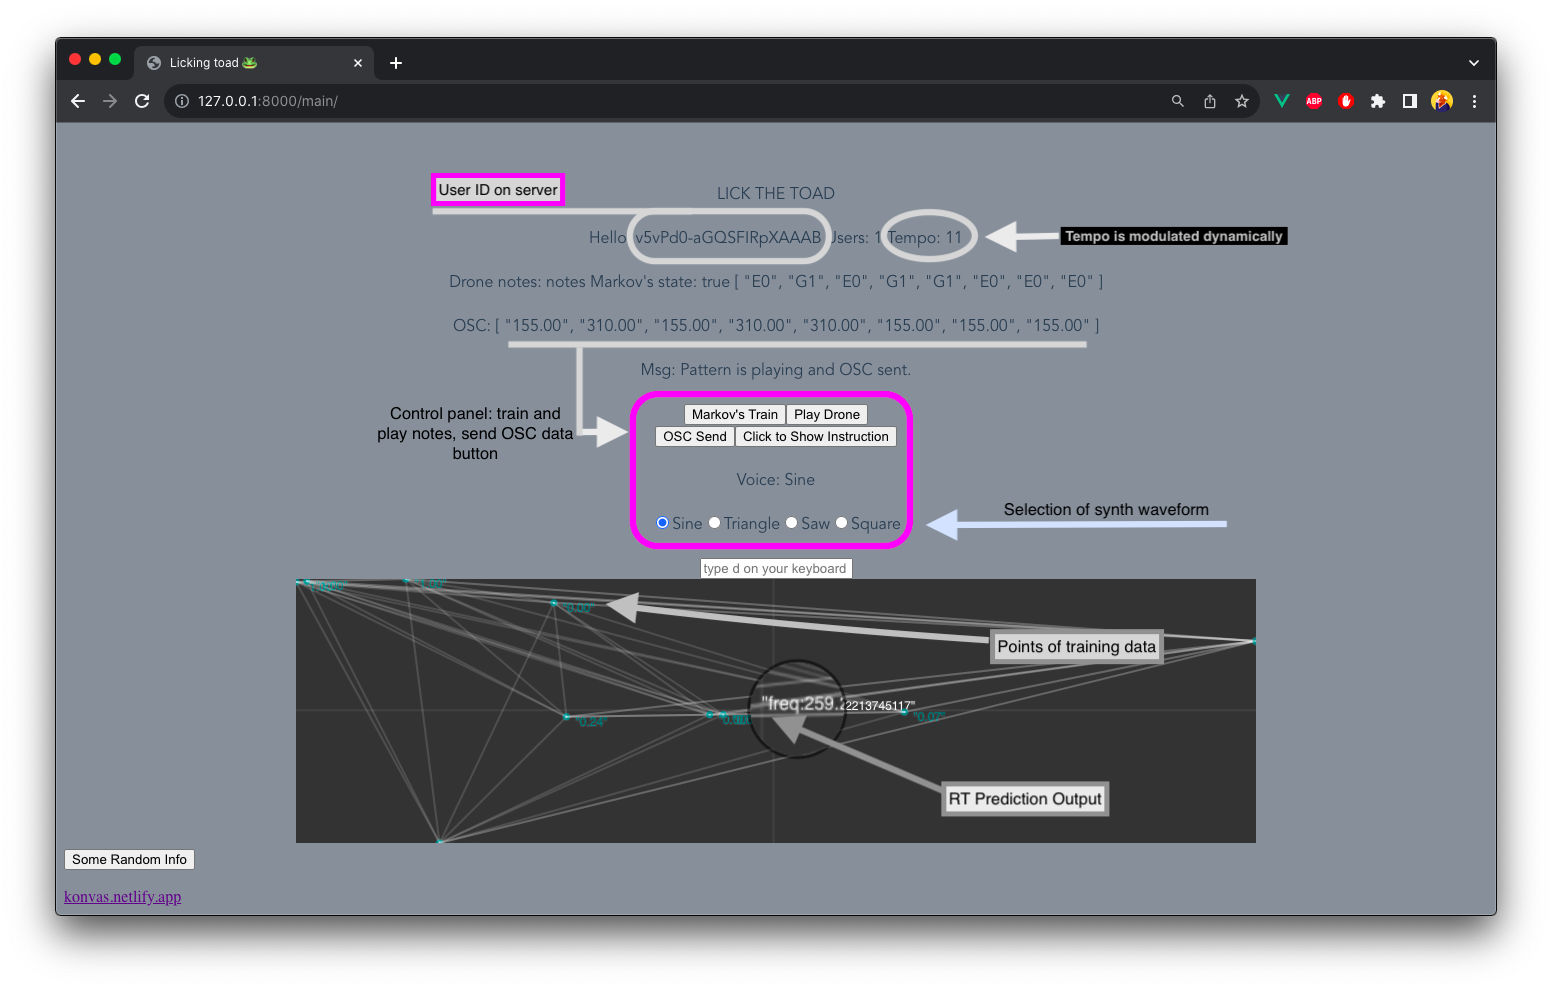
\includegraphics[width=.9\linewidth]{./screens/ltt-interface.png}
\caption{Ltt interface and control GUI.}
\end{figure}
\end{center}
\end{frame}
\section{Development}
\label{sec:org6a18806}
\begin{frame}[label={sec:org5a856e1}]{Technical Details}
\begin{itemize}
\item Project is a client/server system encapsulating training/predictions.
\item Communication client/server is bound through WebSockets, and Express server.
\item Data from clients is using OSCJS library.
\item It is hosted locally with NodeJS and online -> \url{https://lick-the-toad.netlify.app/}
\begin{itemize}
\item Connection with users and OSC is supported only locally now.
\end{itemize}
\item Sound synthesis of clients is using Tone.js and Markov chains extension for JS.
\end{itemize}
\end{frame}
\section{Interaction}
\label{sec:org8130871}
\begin{frame}[label={sec:orgbf2d834}]{Selection of Data on the Fly}
SuperCollider's part of the system supports selection of each event through the user's ID in a GUI.
\begin{center}
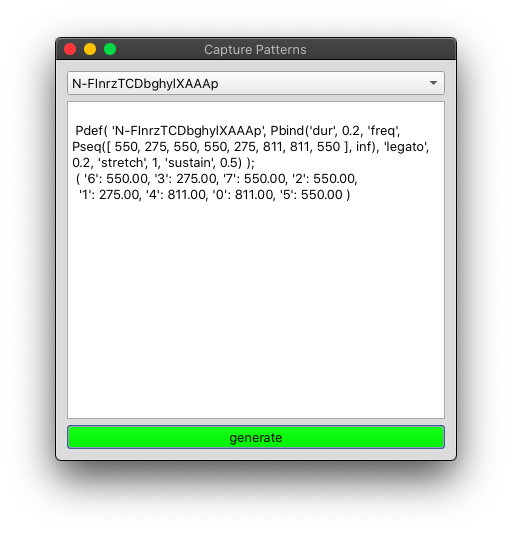
\includegraphics[height=0.5\textwidth]{./screens/sc-pop-up.png}
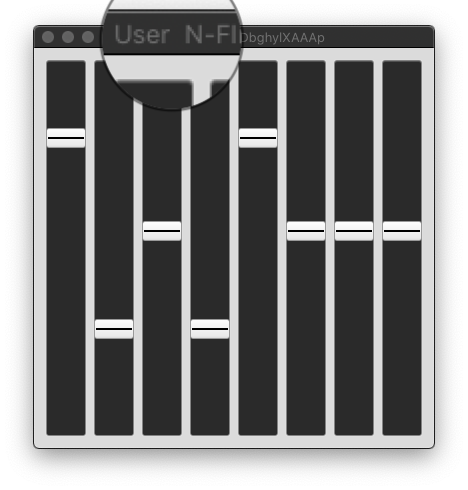
\includegraphics[height=0.5\textwidth]{./screens/sc-sliders.png}
\end{center}
\end{frame}
\section{Network Interaction}
\label{sec:orgc9b9663}
\begin{frame}[label={sec:org68b94df}]{Interoperabillity}
[ "A0", "C4", "C4", "A0", "G2", "G2", "A0", "G2" ]
OSC:[ "214.00", "601.00", "601.00", "214.00", "428.00", "428.00", "214.00", "428.00" ]

The performance is shaped by the data of each user which is interpreted live while the performance unfolds. This way the sounds both from the decentralized domain of the user's together with the live electronics are creating an unpredictable sonic environment which enables the communication between audience and performer.

\begin{itemize}
\item Since the live coding process allows for changing the state of the performance ``instruments'' on the fly, the results can be indeterministic and allow for a wide range of sound outcomes.
\begin{itemize}
\item For this, a plethora of idiomatic interpretation of data to sound is viable, since data is agnostic to music genre and/or textural composition.
\end{itemize}
\end{itemize}
\end{frame}
\section{Sound Making}
\label{sec:org3cde542}
\begin{frame}[label={sec:org9acd6cc},fragile]{Performance Events Patterns and Streams in SC}
 Performance elaborates using Patterns as random or sequential streams, and mapped to any sound parameter:
Examples of patterns include:
\(Prand, Pseq, Pser, Pxrand\)
and more\ldots{}

\begin{itemize}
\item The live coding performance is focussing on the real time sonification of the incoming data.
\item Each user is sending their data in an array of notes.
\item The coder is mapping this values in running processes with the help of streams and patterns of SuperCollider.
\end{itemize}

\begin{verbatim}
Pdef(\user_ID,
	Pbind(\dur, 0.1,
		\freq, Pseq([121.0, 220.0, 340.0, 280], inf)
	));
\end{verbatim}
\end{frame}
\section{Control from SC}
\label{sec:org504a919}
\begin{frame}[label={sec:org9b5ac01},fragile]{SC OSC Interface}
 A small command line is also available from SC to set all users' new states of the Markov chain and trigger back new data. The lines below allow the real time communication with the users interfaces. It triggers the training and the loopback of new data in performer's OSC client.
\begin{verbatim}
n=NetAddr("localhost", 57122);
n.sendMsg('/kv', "markov_train");
n.sendMsg('/kv', "osc_trigger");
\end{verbatim}
\end{frame}
\section{Demo}
\label{sec:org13f32dc}
\begin{frame}[label={sec:orgf6b4e19}]{Demo.}
Live coding in SC -> play some now\ldots{}
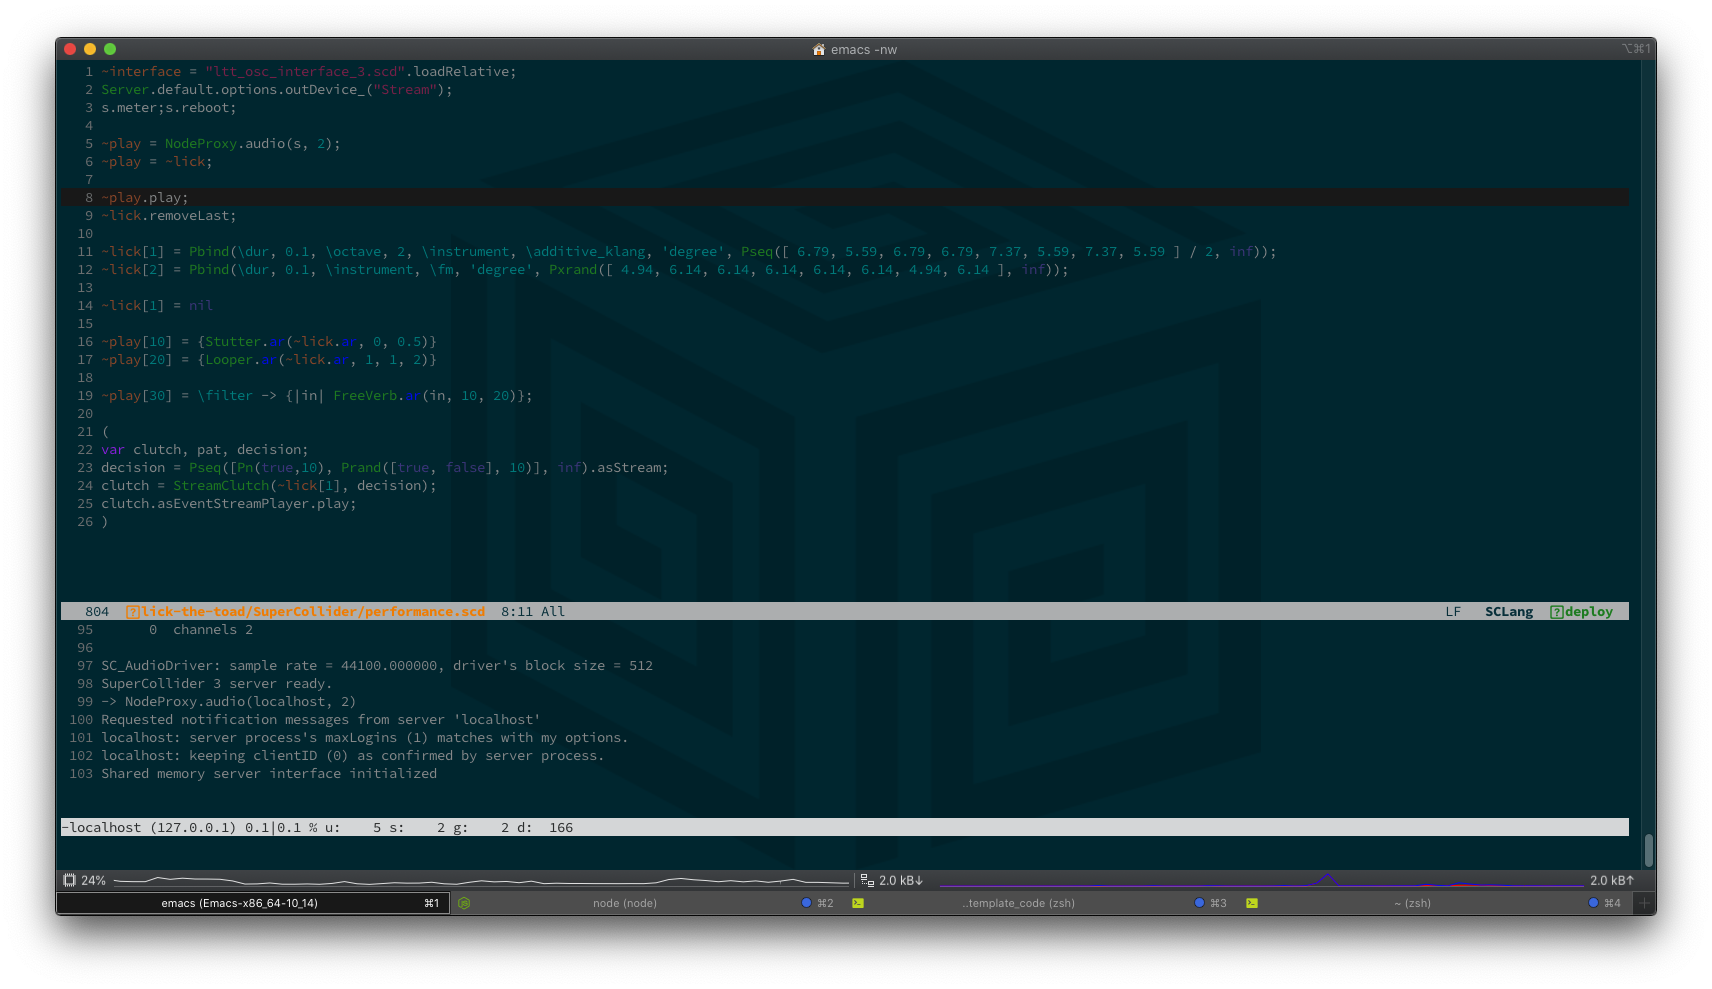
\includegraphics[height=1.0\textwidth]{./screens/live-coding.png}
\end{frame}
\section{Reflections}
\label{sec:orga7678fa}
\begin{frame}[label={sec:org60aa2c8}]{Discussion}
The project aims to serve as an interconnector between coder and audience:

\begin{itemize}
\item Incoming data is the stimuli for real time arbitrary sonifications forming a dynamic soundscape.

\item An unpredictable sound result generated by the algorithm that is trying to connect the gaps by sending proximal values between X and Y coordinates from the user's device.

\item The input serves as the seeding input for a larger chain of processing and interconnection of modules, such as the Markovian chains and the machine learning modules bound together to offer a great paradox of a calculated surprise of unpredictable sonifications.

\item Performer(s) and audience is cooperating throughtout the performance.
\end{itemize}
\end{frame}
\section{Final Remarks}
\label{sec:orgf74fb88}
\begin{frame}[label={sec:org91a7b52}]{Feedback}
Thank you!

\begin{itemize}
\item You may provide your feedback at konstantinos.vasilakos@gmail.com
\end{itemize}
\end{frame}
\end{document}